\documentclass[paper=a4, fontsize=11pt, spanish]{scrartcl}
\usepackage{fourier}
\usepackage{hyperref}

\usepackage{sectsty}
\allsectionsfont{\normalfont\scshape}
\setlength\parindent{0pt}

\usepackage{fancyhdr}
\pagestyle{fancyplain}
\fancyhead{}
\fancyfoot[L]{}
\fancyfoot[C]{}
\fancyfoot[R]{\thepage}
\renewcommand{\headrulewidth}{0pt}
\renewcommand{\footrulewidth}{0pt}
\setlength{\headheight}{13.6pt}

\usepackage[spanish,es-noquoting,es-lcroman]{babel}
\usepackage[utf8]{inputenc}
\usepackage[T1]{fontenc}
\usepackage{graphicx}
\selectlanguage{spanish}

%----------------------------------------------------------------------------------------
%	TÍTULO
%----------------------------------------------------------------------------------------
% Título con las líneas horizontales, nombres y fecha.

\newcommand{\horrule}[1]{\rule{\linewidth}{#1}}

\title{
  \normalfont \normalsize
  \textsc{Universidad de Granada.} \\ [25pt]
  \horrule{0.5pt} \\[0.4cm]
  \huge ERP \\
  \horrule{2pt} \\[0.5cm]
}

\author{Marina Estévez Almenzar\\
\and
Jose Pimentel Mesones\\
\and
Sergio Padilla López\\
\and
Iván Calle Gil\\}

\date{\normalsize\today}


%----------------------------------------------------------------------------------------
%	DOCUMENTO
%----------------------------------------------------------------------------------------

\begin{document}
\maketitle
\newpage

\tableofcontents

\newpage

\section{Introducción}
\subsection{Propósito de este documento}
\setlength{\parindent}{3em} En este documento se describen los requisitos (funcionales y de datos) y las restricciones
semánticas del proyecto para la empresa de diseño web, Emegex Creativos.
\subsection{Convenciones y notación}
\setlength{\parindent}{0em} Utilizaremos la siguiente notación:
\begin{itemize}
\item RF: Requisito funcional
\item RD: Requisito de datos
\item RS: Restricción semántica
\end{itemize}

\subsection{Ámbito de la aplicación}
\setlength{\parindent}{3em} Oficina de Emegex Creativos.

\subsection{Documentos relacionados y referencias}
\begin{itemize}
\item \href{http://emegex.com}{Emegex Creativos}
\item \href{https://github.com/SergioPadilla/ERP}{Repositorio del proyecto}
\end{itemize}

\section{Descripción general}
\subsection{Sistema de información}
\setlength{\parindent}{3em} Vamos a desarrollar un sistema de información para el caso real de una empresa de diseño de páginas web y community manager, en la cual hay un problema de gestión de clientes, de servidores, de dominios y facturación que conlleva una perdida de tiempo para la empresa.

Además, en la empresa se quiere controlar el flujo de trabajo y asignación de tareas entre los empleados.
Para ello, vamos a desarrollar los siguientes módulos:
\begin{itemize}
\item Desarrollo de una base de datos cliente y gestión de los mismos.
\item Desarrollo de una base de datos servidor y otra dominio y gestión de las mismas.
\item Desarrollo de una base de datos facturas y productos y gestión de las facturas.
\item Desarrollo de un “workflow” para la gestión de las tareas entre empleados.
\end{itemize}

\subsection{Usuarios del sistema}
\setlength{\parindent}{0em}Los usuarios del sistema son los empleados de la empresa.

\subsection{Entorno de operación}
\setlength{\parindent}{3em} Desconocido.

\subsection{Restricciones y suposiciones}
\setlength{\parindent}{3em} Los empleados poseen privilegios diferentes, lo que les permite realizar una serie de funcionalidades distintas entre ellos.

\section{Funcionalidad del Sistema}

\subsection{Funcionalidad “Gestión de tareas”}

\subsubsection{Descripción}
\setlength{\parindent}{3em} La gestión de tareas permite una supervisión cómoda y eficiente de una lista de trabajos asignables a los empleados para la estructuración interna de la empresa y el control del trabajo personal y colectivo.

	Para llevar a cabo esta gestión, el administrador crea las tareas y se las asigna a sus empleados (o a él mismo). Además permite asignar una fecha de vencimiento de la tarea, tiempo empleado en llevarla a cabo, registro de horas trabajadas en la misma y comunicación entre administrador y empleado mediante comentarios en la propia tarea.

\subsubsection{Requisitos funcionales}
\setlength{\parindent}{0em}
\textbf{RF1: \textit{Crear tarea}}
\setlength{\parindent}{2em}

Actor: Empleado

Entrada: RD1

Procesamiento: Crea una nueva tarea

Salida: ID tarea

\setlength{\parindent}{0em}
\textbf{RF2: \textit{Añadir subtarea}}
\setlength{\parindent}{2em}

Actor: Empleado

Entrada: RD2

Procesamiento: Añadir tarea a la lista de subtareas

Salida: Ninguna

\setlength{\parindent}{0em}
\textbf{RF3: \textit{Asignar fecha a tarea}}
\setlength{\parindent}{2em}

Actor: Empleado

Entrada: RD3

Procesamiento: Se asigna fecha de vencimiento a la tarea en cuestión

Salida: Ninguna

\setlength{\parindent}{0em}
\textbf{RF4: \textit{Aumentar horas de trabajo en la tarea}}
\setlength{\parindent}{2em}

Actor: Empleado

Entrada: RD4

Procesamiento: Se suman las horas a las ya trabajadas y se restan de las estimadas para completar la tarea

Salida: Ninguna

\setlength{\parindent}{0em}
\textbf{RF5: \textit{Añadir comentario}}
\setlength{\parindent}{2em}

Actor: Empleado

Entrada: RD6

Procesamiento: Añade un comentario a la tarea

Salida: Ninguna

\setlength{\parindent}{0em}
\textbf{RF6: \textit{Borrar comentario}}
\setlength{\parindent}{2em}

Actor: Empleado

Entrada: RD7

Procesamiento: Borra el comentario especificado

Salida: Ninguna

\setlength{\parindent}{0em}
\textbf{RF7: \textit{Asignar tarea}}
\setlength{\parindent}{2em}

Actor: Empleado

Entrada: RD5

Procesamiento: Asignación de tarea a la persona indicada

Salida: Ninguna

\setlength{\parindent}{0em}
\textbf{RF8: \textit{Borrar tarea}}
\setlength{\parindent}{2em}

Actor: Empleado

Entrada: RD2

Procesamiento: Borrar tarea y subtareas indicadas

Salida: Ninguna, o mensaje de error.

\setlength{\parindent}{0em}
\textbf{RF9: \textit{Modificar tarea}}
\setlength{\parindent}{2em}

Actor: Empleado

Entrada: RD8

Procesamiento: Modifica la tarea indicada

Salida: Ninguna, o mensaje de error.

\setlength{\parindent}{0em}
\textbf{RF10: \textit{Listar tareas}}
\setlength{\parindent}{2em}

Actor: Empleado

Entrada: Ninguno

Procesamiento: Lista las tareas

Salida: Tareas listadas

\subsection{Funcionalidad “Gestión de Clientes”}

\subsubsection{Descripción}
\setlength{\parindent}{3em} La gestión de clientes permite manejar de forma cómoda y eficiente los datos de los clientes que han contratado algún servicio con la empresa.

Para llevar a cabo esta gestión, el empleado podrá dar de alta, modificar o borrar clientes, así como consultar la información de los clientes.

\subsubsection{Requisitos funcionales}
\setlength{\parindent}{0em}
\textbf{RF11: \textit{Crear cliente}}
\setlength{\parindent}{2em}

Actor: Empleado

Entrada: RD11

Procesamiento: Crea un nuevo cliente

Salida: RD12

\setlength{\parindent}{0em}
\textbf{RF12: \textit{Borrar cliente}}
\setlength{\parindent}{2em}

Actor: Empleado

Entrada: RD13

Procesamiento:Se elimina los datos relacionados con el cliente de ID especificada

Salida: Ninguna (si no existe el ID, devuelve mensaje de error)

\setlength{\parindent}{0em}
\textbf{RF13: \textit{Modificar cliente}}
\setlength{\parindent}{2em}

Actor: Empleado

Entrada: RD13, RD14

Procesamiento: Se modifica los datos asociados al cliente con ID especificado en RD13

Salida: Ninguna (si no existe el ID, devuelve mensaje de error)

\setlength{\parindent}{0em}
\textbf{RF14: \textit{Consultar cliente}}
\setlength{\parindent}{2em}

Actor: Empleado

Entrada: RD13

Procesamiento: Se muestra la información almacenado del cliente con identificador proporcionado por RD13

Salida:  RD12 (si no existe el ID, devuelve mensaje de error)

\setlength{\parindent}{0em}
\textbf{RF15: \textit{Clasificar clientes}}
\setlength{\parindent}{2em}

Actor: Empleado

Entrada: RD15

Procesamiento:  Se busca entre todos los clientes almacenados aquellos que cumplan las condiciones impuestas por RD5

Salida: RD6 (pudiendo aparecer una lista vacia)

\subsection{Funcionalidad “Gestión de facturas y productos”}

\subsubsection{Descripción}
\setlength{\parindent}{3em} La gestión de facturas y productos permite a la empresa un seguimiento fiable y un control eficiente de los productos ofrecidos por la misma, a la vez que proporciona una buena ordenación de las facturas emitidas en la compra de dichos productos. Como consecuencia, esta gestión también proporcionará las relaciones que se establecen entre los productos y las facturas.

	Para llevar a cabo esta gestión, se crearán los productos que desea ofrecer al cliente, añadiendo la opción de poder consultarlos, modificarlos e incluso eliminarlos de la lista de productos ofrecidos. En cuanto a las facturas se gestionarán igual. Cabe la posibilidad de añadir la opción de impresión de facturas.

\subsubsection{Requisitos funcionales}
\setlength{\parindent}{0em}
	\textbf{RF16: \textit{Crear producto}}
	\setlength{\parindent}{2em}

	Actor: Empleado

	Entrada: RD17

	Procesamiento: Crea un nuevo producto

	Salida: Ninguna (si falta algún dato de entrada, devuelve un mensaje de error)

	\setlength{\parindent}{0em}
	\textbf{RF17: \textit{Consultar producto}}
	\setlength{\parindent}{2em}

	Actor: Empleado

	Entrada: RD18

	Procesamiento: Consultar el estado de un producto

	Salida: ID, nombre, descripción, importe del producto, número de ventas (si el producto no existe, devuelve un mensaje de error)

	\setlength{\parindent}{0em}
	\textbf{RF18: \textit{Modificar producto}}
	\setlength{\parindent}{2em}

	Actor: Empleado

	Entrada: RD19

	Procesamiento: Se modifican los datos del producto en cuestión

	Salida: Ninguna (si el producto no existe, devuelve un mensaje de error)

	\setlength{\parindent}{0em}
	\textbf{RF19: \textit{Ordenar productos}}
	\setlength{\parindent}{2em}

	Actor: Empleado

	Entrada: Ninguna

	Procesamiento: Ordena los productos del más vendido al menos vendido

	Salida: Lista de productos (ID y nombre del producto)

	\setlength{\parindent}{0em}
	\textbf{RF20: \textit{Eliminar producto}}
	\setlength{\parindent}{2em}

	Actor: Empleado

	Entrada: RD20

	Procesamiento: Se elimina el producto en cuestión del conjunto de productos

	Salida: Ninguna (si el producto no existe, devuelve un mensaje de error)

	\setlength{\parindent}{0em}
	\textbf{RF21: \textit{Crear factura}}
	\setlength{\parindent}{2em}

	Actor: Empleado

	Entrada: RD21

	Procesamiento: Crea una factura de la compra de algún cliente

	Salida: Ninguna (si falta algún dato de entrada, devuelve un mensaje de error)

	\setlength{\parindent}{0em}
	\textbf{RF22: \textit{Consultar factura}}
	\setlength{\parindent}{2em}

	Actor: Empleado

	Entrada: RD22

	Procesamiento: Consulta una de las facturas ya creadas

	Salida: ID de factura, cliente correspondiente, fecha de emisión e importe total

	\setlength{\parindent}{0em}
	\textbf{RF23: \textit{Imprimir factura (opcional)}}
	\setlength{\parindent}{2em}

	Actor: Empleado

	Entrada: RD23

	Procesamiento: Se imprime la factura en cuestión

	Salida: Ninguna (si la factura no existe, devuelve un mensaje de error)

\subsection{Funcionalidad “Gestión de Servidores y Dominios”}

\subsubsection{Descripción}
\setlength{\parindent}{3em} En esta funcionalidad se intenta solucionar el problema de almacenar de forma segura y ordenar de forma eficiente los datos referentes a los servidores y dominios del cliente, para que la empresa pueda acceder a esta información en el menor tiempo posible y así aumentar la productividad.

Para solucionar este problema, los empleados podrán crear un servidor en la base de datos asociado a un cliente y crear dominios asociados a un servidor, también se podrá modificar los datos del servidor y de los dominios ya creados. Se podrán consultar los datos de los servidores y de los dominios pero solo el administrador podrá borrar los datos.

\subsubsection{Requisitos funcionales}
\setlength{\parindent}{0em}
\textbf{RF24:\textit{Crear servidor}}
\setlength{\parindent}{3em}

Actor: Empleado

Entrada: RD27

Procesamiento: Crea un nuevo servidor encriptando las contraseñas

Salida: ID servidor

\setlength{\parindent}{0em}
\textbf{RF25:\textit{Consultar servidor}}
\setlength{\parindent}{3em}

Actor: Empleado

Entrada: RD28

Procesamiento: Consultar el estado de un servidor desencriptando contraseñas

Salida: ID servidor, ID cliente, nombre del servidor, url o ip de acceso, usuario (ftp),contraseña (ftp), usuario(host),contraseña(host)(si el servidor no existe, devuelve un mensaje de error)

\setlength{\parindent}{0em}
\textbf{RF26:\textit{Modificar servidor}}
\setlength{\parindent}{3em}

Actor: Empleado

Entrada: RD29

Procesamiento: Se modifican los datos del servidor si modifica la contraseña encriptar

Salida: Ninguna (si el servidor no existe, devuelve un mensaje de error)

\setlength{\parindent}{0em}
\textbf{RF27:\textit{Listar servidores}}
\setlength{\parindent}{3em}

Actor: Empleado

Entrada: RD30

Procesamiento: Lista los servidores de un cliente

Salida: Lista de servidores(nombre del del servidor)

\setlength{\parindent}{0em}
\textbf{RF28:\textit{Borrar servidor}}
\setlength{\parindent}{3em}

Actor: Empleado

Entrada: RD28

Procesamiento: Se elimina los datos del servidor

Salida: Ninguna  (si el servidor no existe, devuelve un mensaje de error)

\setlength{\parindent}{0em}
\textbf{RF29:\textit{Crear dominio}}
\setlength{\parindent}{3em}

Actor: Empleado

Entrada: RD31

Procesamiento: Crea crea un dominio asociado a un servidor

Salida: ID del dominio

\setlength{\parindent}{0em}
\textbf{RF30:\textit{Consultar dominio}}
\setlength{\parindent}{3em}

Actor: Empleado

Entrada: RD32

Procesamiento: Consulta un dominio

Salida: ID dominio, ID servidor, Dirección web

\setlength{\parindent}{0em}
\textbf{RF31:\textit{Borrar dominio}}
\setlength{\parindent}{3em}

Actor: Empleado

Entrada: RD32

Procesamiento: Se eliminan los datos del dominio en la base de datos.

Salida: Ninguna  (si el dominio no existe, devuelve un mensaje de error)

\section{Requisitos de datos}
\setlength{\parindent}{0em}
\textbf{RD1: \textit{Datos opcionales para crear una tarea}}
\setlength{\parindent}{2em}
\begin{itemize}
\item Título [cadena de caracteres]
\item Descripción [Cadena de caracteres]
\item Tiempo estimado [número real]
\end{itemize}

\setlength{\parindent}{0em}
\textbf{RD2: \textit{Datos necesarios para identificar una tarea}}
\setlength{\parindent}{2em}
\begin{itemize}
\item ID tarea
\end{itemize}

\setlength{\parindent}{0em}
\textbf{RD3: \textit{Datos necesarios para asignar fecha a una tarea}}
\setlength{\parindent}{2em}
\begin{itemize}
\item Fecha
\end{itemize}

\setlength{\parindent}{0em}
\textbf{RD4: \textit{Datos necesarios para aumentar las horas de trabajo en una tarea}}
\setlength{\parindent}{2em}
\begin{itemize}
\item Horas trabajadas
\end{itemize}

\setlength{\parindent}{0em}
\textbf{RD5: \textit{Datos necesarios para asignar tarea}}
\setlength{\parindent}{2em}
\begin{itemize}
\item ID empleado
\end{itemize}

\setlength{\parindent}{0em}
\textbf{RD6: \textit{Datos necesarios para añadir comentario}}
\setlength{\parindent}{2em}
\begin{itemize}
\item Comentario [cadena de texto]
\end{itemize}

\setlength{\parindent}{0em}
\textbf{RD7: \textit{Datos necesarios para borrar comentario}}
\setlength{\parindent}{2em}
\begin{itemize}
\item ID comentario
\end{itemize}

\setlength{\parindent}{0em}
\textbf{RD8: \textit{Datos almacenados en TAREAS}}
\setlength{\parindent}{2em}
\begin{itemize}
\item ID tarea
\item Título
\item Fecha de vencimiento
\item ID tarea\_padre
\item Horas estimadas
\item ID empleado\_asignado
\item Estado
\item Descripción
\end{itemize}

\setlength{\parindent}{0em}
\textbf{RD9: \textit{Datos almacenados en COMENTARIOS}}
\setlength{\parindent}{2em}
\begin{itemize}
\item ID comentario
\item texto [cadena de caracteres]
\item ID Tarea
\end{itemize}

\setlength{\parindent}{0em}
\textbf{RD10: \textit{Datos almacenados en REGISTROS}}
\setlength{\parindent}{2em}
\begin{itemize}
\item ID registro
\item ID empleado
\item Horas trabajadas
\item Descripción [cadena de texto]
\item Fecha
\end{itemize}

\setlength{\parindent}{0em}
\textbf{RD11: \textit{ Datos necesarios para crear un nuevo cliente}}
\setlength{\parindent}{2em}
\begin{itemize}
\item Tipo [cadena de caracteres]
\item Nombre / Nombre Comercial [Cadena de caracteres]
\item Apellido / Nombre Fiscal [Cadena de caracteres]
\item NIF / CIF [Cadena de caracteres]
\item Correo electrónico [Cadena de caracteres]
\end{itemize}

\setlength{\parindent}{0em}
\textbf{RD12: \textit{Datos almacenados CLIENTES}}
\setlength{\parindent}{2em}
\begin{itemize}
\item ID cliente
\item Tipo [cadena de caracteres]
\item Nombre / Nombre Comercial [Cadena de caracteres]
\item Apellido / Nombre Fiscal [Cadena de caracteres]
\item NIF / CIF [Cadena de caracteres]
\item Correo electrónico [Cadena de caracteres]
\item Fecha de alta
\end{itemize}

\setlength{\parindent}{0em}
\textbf{RD13: \textit{Datos necesarios para acceder a cliente}}
\setlength{\parindent}{2em}
\begin{itemize}
\item ID tarea
\end{itemize}

\setlength{\parindent}{0em}
\textbf{RD14: \textit{Datos necesarios para modificar el cliente}}
\setlength{\parindent}{2em}
\begin{itemize}
\item Tipo [cadena de caracteres]
\item Nombre / Nombre Comercial [Cadena de caracteres]
\item Apellido / Nombre Fiscal [Cadena de caracteres]
\item NIF / CIF [Cadena de caracteres]
\item Correo electrónico [Cadena de caracteres]
\end{itemize}

\setlength{\parindent}{0em}
\textbf{RD15: \textit{Parametros por los que clasificar nuestra lista de clientes}}
\setlength{\parindent}{2em}
\begin{itemize}
\item Tipo [cadena de caracteres]
\item Nombre / Nombre Comercial [Cadena de caracteres]
\item Apellido / Nombre Fiscal [Cadena de caracteres]
\item NIF / CIF [Cadena de caracteres]
\item Correo electrónico [Cadena de caracteres]
\item fecha de alta
\end{itemize}

\setlength{\parindent}{0em}
\textbf{RD16: \textit{Lista de identificadores clientes}}
\setlength{\parindent}{2em}
\begin{itemize}
\item Lista de clientes [Lista de IDs de clientes]
\end{itemize}

\setlength{\parindent}{0em}
	\textbf{RD17: \textit{Datos necesarios para crear un producto}}
	\setlength{\parindent}{2em}
	\begin{itemize}
		\item Nombre del producto [cadena de caracteres]
		\item Descripción [cadena de caracteres]
		\item Importe
	\end{itemize}

	\setlength{\parindent}{0em}
	\textbf{RD18: \textit{Datos necesarios para consultar un producto}}
	\setlength{\parindent}{2em}
	\begin{itemize}
		\item ID del producto
	\end{itemize}

	\setlength{\parindent}{0em}
	\textbf{RD19: \textit{Datos necesarios para modificar un producto}}
	\setlength{\parindent}{2em}
	\begin{itemize}
		\item ID del producto
		\item Dato a modificar (nombre del producto, descripción, importe)
	\end{itemize}

	\setlength{\parindent}{0em}
	\textbf{RD20: \textit{Datos necesarios para eliminar un producto}}
	\setlength{\parindent}{2em}
	\begin{itemize}
		\item ID de producto
	\end{itemize}

	\setlength{\parindent}{0em}
	\textbf{RD21: \textit{Datos necesarios para crear una factura}}
	\setlength{\parindent}{2em}
	\begin{itemize}
		\item ID del cliente involucrado
	\end{itemize}

	\setlength{\parindent}{0em}
	\textbf{RD22: \textit{Datos necesarios para consultar una factura}}
	\setlength{\parindent}{2em}
	\begin{itemize}
		\item ID de factura
	\end{itemize}

	\setlength{\parindent}{0em}
	\textbf{RD23: \textit{Datos necesarios para imprimir una factura}}
	\setlength{\parindent}{2em}
	\begin{itemize}
		\item ID de factura
	\end{itemize}

	\setlength{\parindent}{0em}
	\textbf{RD24: \textit{Datos almacenados en PRODUCTOS}}
	\setlength{\parindent}{2em}
	\begin{itemize}
		\item ID de producto
		\item Nombre del producto [cadena de caracteres]
		\item Descripción [cadena de caracteres]
		\item Importe [número real]
		\item Número de ventas [número entero]
	\end{itemize}

	\setlength{\parindent}{0em}
	\textbf{RD25: \textit{Datos almacenados en FACTURAS}}
	\setlength{\parindent}{2em}
	\begin{itemize}
		\item ID de factura
		\item Fecha de emisión
		\item ID cliente involucrado
		\item Importe total [número real]
	\end{itemize}

	\setlength{\parindent}{0em}
	\textbf{RD26: \textit{Datos almacenados en COMPRAS}}
	\setlength{\parindent}{2em}
	\begin{itemize}
		\item ID de factura
		\item ID de producto
		\item Precio
	\end{itemize}

\setlength{\parindent}{0em}
\textbf{RD27: \textit{Datos necesarios para crear un servidor}}
\setlength{\parindent}{2em}
\begin{itemize}
  \item ID cliente [número entero]
  \item Nombre del servidor [cadena de caracteres]
  \item Url o ip de acceso [cadena de caracteres]
  \item usuario (ftp) [cadena de caracteres]
  \item contraseña (ftp) [cadena de caracteres]
  \item usuario (host) [cadena de caracteres]
  \item contraseña (host) [cadena de caracteres]
\end{itemize}

\setlength{\parindent}{0em}
\textbf{RD28: \textit{Datos necesarios para consultar un servidor}}
\setlength{\parindent}{2em}
\begin{itemize}
  \item ID servidor
\end{itemize}

\setlength{\parindent}{0em}
\textbf{RD29: \textit{Datos necesarios para modificar un servidor}}
\setlength{\parindent}{2em}
\begin{itemize}
  \item ID del servidor
  \item Nuevo dato (ID cliente, nombre del servidor, url o ip de acceso, usuario (ftp),contraseña (ftp), usuario(host),contraseña(host))
\end{itemize}

\setlength{\parindent}{0em}
\textbf{RD30: \textit{Datos necesarios para listar servidores}}
\setlength{\parindent}{2em}
\begin{itemize}
  \item ID cliente
\end{itemize}

\setlength{\parindent}{0em}
\textbf{RD31: \textit{Datos necesarios para crear dominio}}
\setlength{\parindent}{2em}
\begin{itemize}
  \item ID servidor
  \item Dirección web
\end{itemize}

\setlength{\parindent}{0em}
\textbf{RD32: \textit{Datos necesarios para consultar dominio}}
\setlength{\parindent}{2em}
\begin{itemize}
  \item ID dominio
\end{itemize}

\setlength{\parindent}{0em}
\textbf{RD33: \textit{Datos almacenados en SERVIDORES}}
\setlength{\parindent}{2em}
\begin{itemize}
  \item ID servidor [número entero]
  \item ID cliente [número entero]
  \item nombre del servidor [cadena de caracteres]
  \item url o ip de acceso [cadena de caracteres]
  \item usuario (ftp) [cadena de caracteres]
  \item contraseña (ftp) [cadena de caracteres]
  \item usuario(host) [cadena de caracteres]
  \item contraseña(host) [cadena de caracteres]
\end{itemize}

\setlength{\parindent}{0em}
\textbf{RD34: \textit{Datos almacenados en DOMINIOS}}
\setlength{\parindent}{2em}
\begin{itemize}
  \item ID dominio [número entero]
  \item ID servidor [número entero]
  \item Dirección web [cadena de caracteres]
\end{itemize}

\setlength{\parindent}{0em}
\textbf{RD35: \textit{Datos almacenados en EMPLEADOS}}
\setlength{\parindent}{2em}
\begin{itemize}
  \item ID empleado
  \item DNI
  \item Nombre
  \item Apellidos
  \item permiso
\end{itemize}

\section{Restricciones Semánticas}
\setlength{\parindent}{0em}
\textbf{RS1: \textit{Tareas y subtareas}}
\setlength{\parindent}{2em}

Las subtareas son tareas en sí, tienen su propia id, diferente de la tarea de la que dependen la cual se refleja en la base de datos para saber que es subtarea.

\setlength{\parindent}{0em}
\textbf{RS2: \textit{Asignación de tareas}}
\setlength{\parindent}{2em}

Cualquier empleado puede asignar tareas.

\setlength{\parindent}{0em}
\textbf{RS3: \textit{Permisos de empleado}}
\setlength{\parindent}{2em}

Tipos de permisos:
\begin{itemize}
\item 1: Permiso de administrador (sin restricciones)
\item 2: Permiso para gestionar facturas y productos: Puede crearlos y modificarlos.
\item 3: Permiso para gestionar servidores: Puede crearlos y modificarlos.
\item 4: Permiso para gestionar clientes: Puede crearlos y modificar sus datos.
\item 5: Solo puede utilizar la funcionalidad relacionada con las tareas.
\end{itemize}

\setlength{\parindent}{0em}
\textbf{RS4: \textit{Relación de permisos de empleados}}
\setlength{\parindent}{2em}

A menor número de permiso, mayor privilegio, es decir, el empleado con tipo de privilegio 1 posee todos los permisos, heredando los privilegios de tipos posteriores.
Ejemplo: un empleado con tipo de privilegio 3, posee los privilegios de tipo 4 y 5 por defecto.

\setlength{\parindent}{0em}
\textbf{RS5: \textit{Creación y modificación de clientes}}
\setlength{\parindent}{2em}

Los empleados con privilegios tipo menor o igual que 4 son los que pueden crear y modificar clientes, además el campo de tipo de cliente jamás puede quedar sin rellenar, el resto no poseen este tipo de restricciones.


\setlength{\parindent}{0em}
\textbf{RS6: \textit{Eliminación de clientes}}
\setlength{\parindent}{2em}

El empleado con tipo de privilegio 1 es el único que puede eliminar clientes.

\setlength{\parindent}{0em}
\textbf{RS7: \textit{Tipos de clientes}}
\setlength{\parindent}{2em}

Un cliente puede ser tipo empresa, y entonces tendrá relleno los datos de NIF y de nombre comercial, o ser tipo autónomo, en cuyo caso recogeremos los datos de nombre, apellidos y DNI, lugar de los mencionados anteriormente. El resto de datos son comunes para ambos tipos de clientes.

\setlength{\parindent}{0em}
\textbf{RS8: \textit{Consultar clientes}}
\setlength{\parindent}{2em}

Cualquier empleado puede consultar la información sobre los clientes.

\setlength{\parindent}{0em}
\textbf{RS9: \textit{Crear y modificar productos}}
\setlength{\parindent}{2em}

Los empleados con tipo de privilegio menor o igual que 2 son los únicos que pueden crear y modificar productos.

\setlength{\parindent}{0em}
\textbf{RS10: \textit{Eliminar productos}}
\setlength{\parindent}{2em}

Los empleados con tipo de privilegio 1 son los únicos que pueden eliminar productos.

\setlength{\parindent}{0em}
\textbf{RS11: \textit{Consultar y ordenar productos}}
\setlength{\parindent}{2em}

Cualquier empleado puede consultar y ordenar productos.

\setlength{\parindent}{0em}
\textbf{RS12: \textit{Crear y modificar facturas}}
\setlength{\parindent}{2em}

Los empleados con tipo de privilegio menor o igual que 2 son los únicos que pueden crear y modificar facturas.

\setlength{\parindent}{0em}
\textbf{RS13: \textit{Consultar e imprimir facturas}}
\setlength{\parindent}{2em}

Cualquier empleado puede consultar e imprimir facturas.

\setlength{\parindent}{0em}
\textbf{RS14: \textit{Facturas y productos eliminados}}
\setlength{\parindent}{2em}

Al eliminar un producto, no desaparecen las posibles relaciones que tenga dicho producto con las facturas de compras anteriores del mismo: el producto eliminado no desaparece de la tabla que relaciona cada factura con los productos involucrados.

\setlength{\parindent}{0em}
\textbf{RS15: \textit{Creación y modificación de servidores y dominios}}
\setlength{\parindent}{2em}

Los empleados con tipo de privilegio menor o igual que 3 son los únicos que pueden crear y modificar servidores y dominios.

\setlength{\parindent}{0em}
\textbf{RS16: \textit{Consultar y listar servidores}}
\setlength{\parindent}{2em}

Cualquier empleado puede consultar y listar servidores.

\setlength{\parindent}{0em}
\textbf{RS17: \textit{Elminiar dominios}}
\setlength{\parindent}{2em}

Los empleados con tipo de privilegio 1 son los únicos capaces de eliminar dominios.

\setlength{\parindent}{0em}
\textbf{RS18: \textit{Consultar dominios y servidores}}
\setlength{\parindent}{2em}

Cualquier empleado puede consultar dominios y servidores.

\setlength{\parindent}{0em}
\textbf{RS19: \textit{servidores y dominios eliminados}}
\setlength{\parindent}{2em}

Al eliminar un servidor se eliminaran también los dominios asociados a ese servidor, pero si se elimina un dominio, solo se elimina el dominio.

\setlength{\parindent}{0em}
\textbf{RS20: \textit{Estado de las tareas}}
\setlength{\parindent}{2em}

El estado de cada tarea puede ser uno de los tres siguientes: 'por hacer', 'en desarrollo' o 'hecho'.

\section{Diseño Físico}
\subsection{CLIENTES}
CREATE TABLE clientes (id\_cliente INT NOT NULL PRIMARY KEY AUTO\_INCREMENT, tipo ENUM(‘particular’, ‘empresa’),  nombre TEXT,  apellido TEXT, nif varchar(10) UNIQUE , email TEXT, fecha\_alta DATETIME)

\subsection{PRODUCTOS}
CREATE TABLE productos (id\_producto INT NOT NULL PRIMARY KEY AUTO\_INCREMENT, nombre TEXT,  descripcion TEXT,  importe FLOAT, ventas INT DEFAULT 0)

\subsection{FACTURAS}
CREATE TABLE facturas (id\_factura INT NOT NULL PRIMARY KEY AUTO\_INCREMENT, fecha DATETIME, id\_cliente INT REFERENCES clientes (id\_cliente))

\subsection{COMPRAS}
CREATE TABLE compras (id\_producto INT REFERENCES productos (id\_producto), id\_factura INT REFERENCES facturas (id\_factura), precio FLOAT, PRIMARY KEY(id\_producto,id\_factura))

\subsection{SERVIDORES}
CREATE TABLE servidores (id\_servidor INT NOT NULL PRIMARY KEY AUTO\_INCREMENT, id\_cliente INT REFERENCES clientes (id\_cliente), nombre TEXT,  ruta\_de\_acceso TEXT, usuario\_ftp TEXT, password\_ftp TEXT, usuario\_host TEXT, password\_host TEXT)

\subsection{DOMINIOS}
CREATE TABLE dominios (id\_dominio INT NOT NULL PRIMARY KEY AUTO\_INCREMENT, id\_servidor INT REFERENCES servidores (id\_servidor), web TEXT)

\subsection{EMPLEADOS}
CREATE TABLE empleados (id\_empleado INT NOT NULL PRIMARY KEY AUTO\_INCREMENT, dni varchar(9) UNIQUE NOT NULL,  nombre TEXT, password TEXT, apellidos TEXT, permisos INT)

\subsection{TAREAS}
CREATE TABLE tareas (id\_tarea INT NOT NULL PRIMARY KEY AUTO\_INCREMENT, titulo TEXT, fecha DATE, descripcion TEXT, id\_tarea\_padre INT, horas\_estimadas TIME, empleado\_asignado INT REFERENCES empleados (id\_empleado), estado ENUM('TO\_DO', 'DEVELOPMENT', 'DONE'))

\subsection{REGISTROS}
CREATE TABLE registros (id\_registro INT NOT NULL PRIMARY KEY AUTO\_INCREMENT, id\_empleado INT REFERENCES empleados (id\_empleado), horas\_trabajadas TIME, descripción TEXT, fecha DATE)

\subsection{COMENTARIOS}
CREATE TABLE comentarios (id\_comentario INT NOT NULL PRIMARY KEY AUTO\_INCREMENT, texto TEXT, tarea INT REFERENCES tareas (id\_tarea))

\subsection{ROL}
CREATE TABLE rol (rol INT NOT NULL , permiso INT, PRIMARY KEY(rol,permiso))


\section{DISEÑO}
\subsection {Diagrama de flujo de datos y esquemas externos}
\subsubsection* {Esquema de caja negra: ~\ref{fig:cajanegra}}
\subsubsection* {Diagrama armazón F: ~\ref{fig:armazonF}}
\subsubsection* {Esquemas externos para el diagrama armazón F: ~\ref{fig:exArmazonF}}
\subsubsection* {Diagrama armazón D: ~\ref{fig:armazonD}}
\subsubsection* {Primer refinamiento del diagrama F: ~\ref{fig:primerRefF}}
\subsubsection* {Esquemas externos del plano de refinamiento F: ~\ref{fig:EsqExtF}}
\subsubsection* {Primer refinamiento del diagrama D: ~\ref{fig:PrimerRefD}}
\subsubsection* {Segundo refinamiento del diagrama F: ~\ref{fig:SegundoRefF}}
\subsubsection* {Esquemas externos del plano de refinamiento F: ~\ref{fig:EsqExtF_2}}
\subsubsection* {Segundo refinamiento del diagrama D: ~\ref{fig:SegundoRefD}}
\subsubsection* {Plano final: ~\ref{fig:PlanoFinal}}


\begin{figure}
	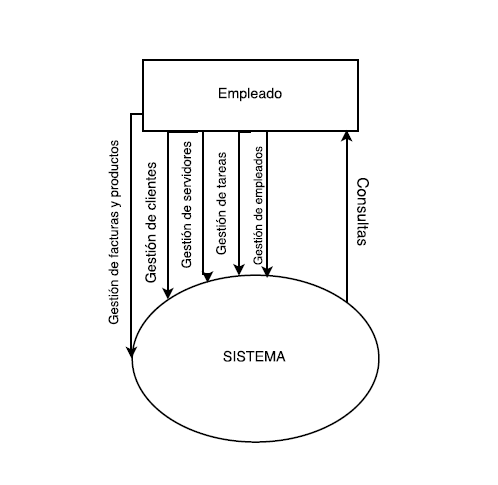
\includegraphics{ERP_EMEGEX.png}
	\caption{}
	\label{fig:cajanegra}
\end{figure}

\begin{figure}
	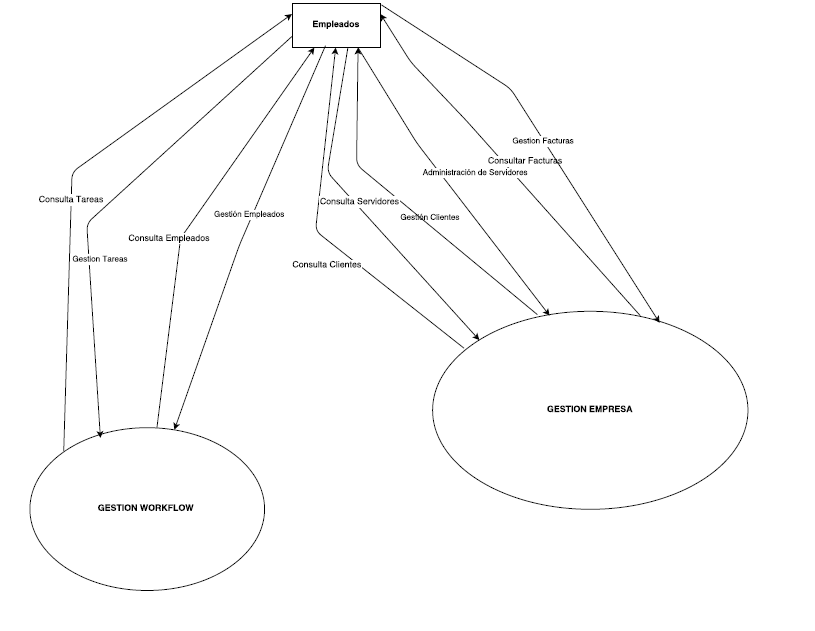
\includegraphics[width=1.25\textwidth]{ArmazonF.png}
	\caption{}
	\label{fig:armazonF}
\end{figure}

\begin{figure}
	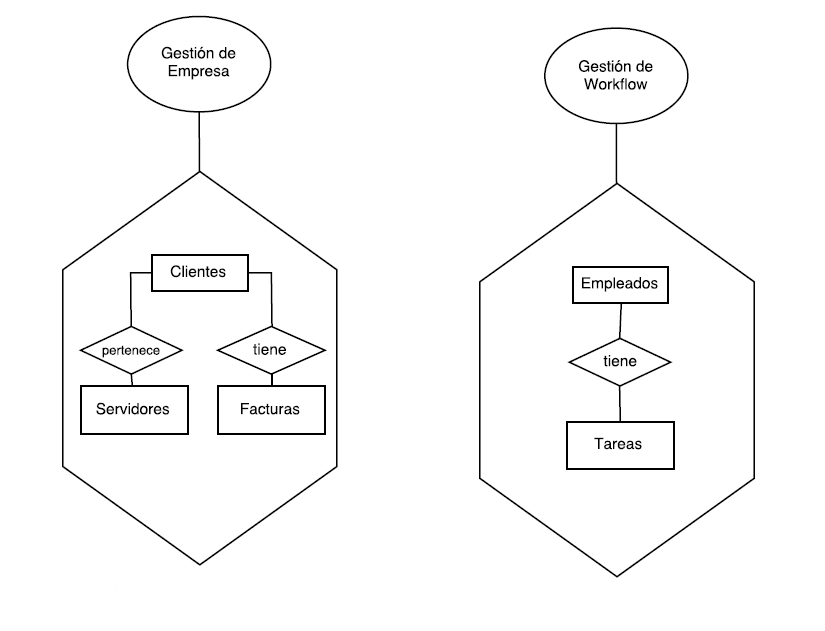
\includegraphics[width=1.25\textwidth]{exArmazonF.png}
	\caption{}
	\label{fig:exArmazonF}
\end{figure}

\begin{figure}
	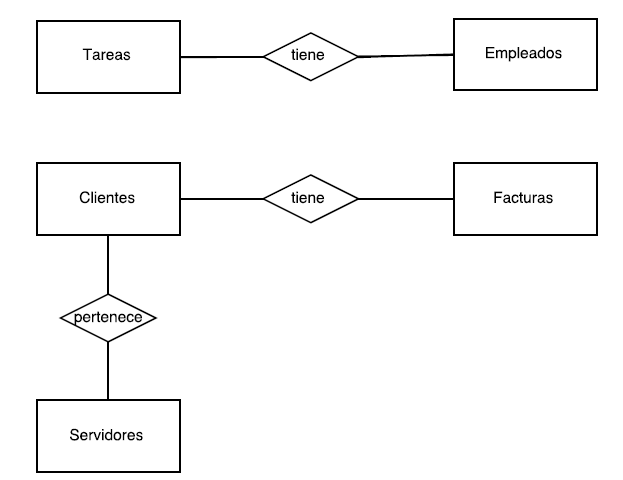
\includegraphics{ArmazonD.png}
	\caption{}
	\label{fig:armazonD}
\end{figure}

\begin{figure}
	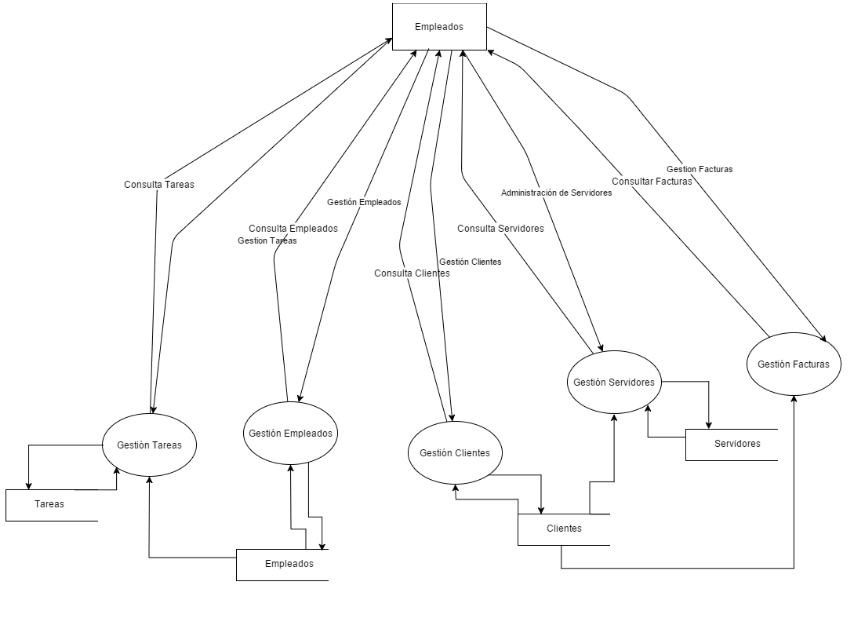
\includegraphics[width=1.20\textwidth]{PrimerRefF.png}
	\caption{}
	\label{fig:primerRefF}
\end{figure}

\begin{figure}
	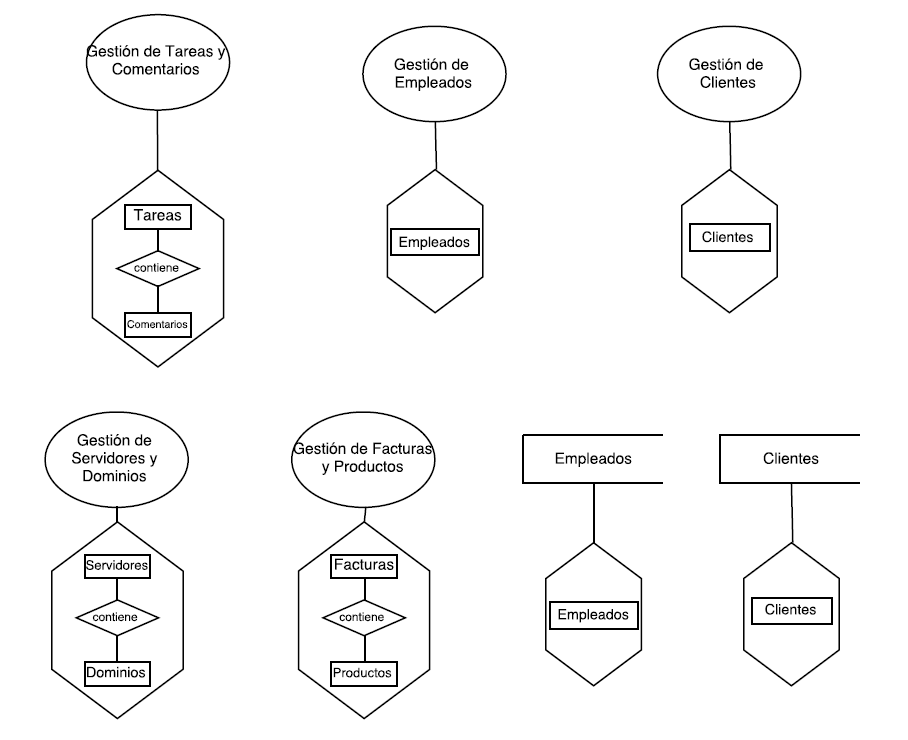
\includegraphics[width=1.25\textwidth]{EsqExtF.png}
	\caption{}
	\label{fig:EsqExtF}
\end{figure}

\begin{figure}
	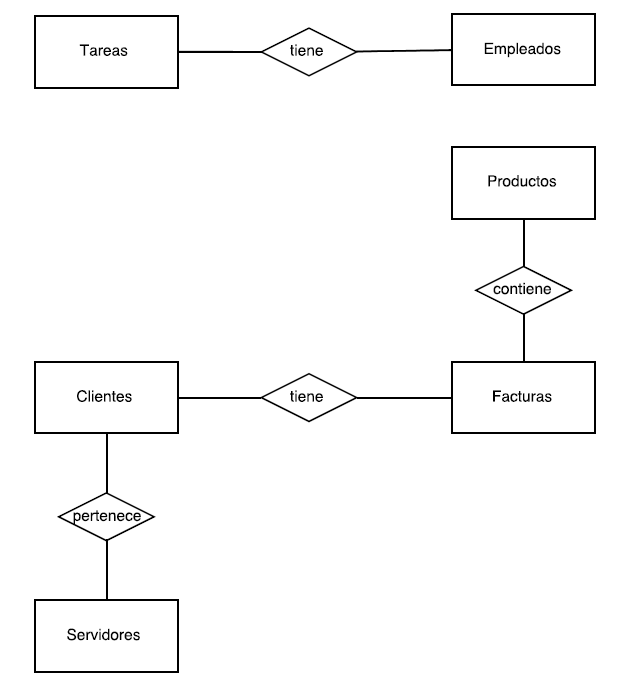
\includegraphics{PrimerRefD.png}
	\caption{}
	\label{fig:PrimerRefD}
\end{figure}

\begin{figure}
	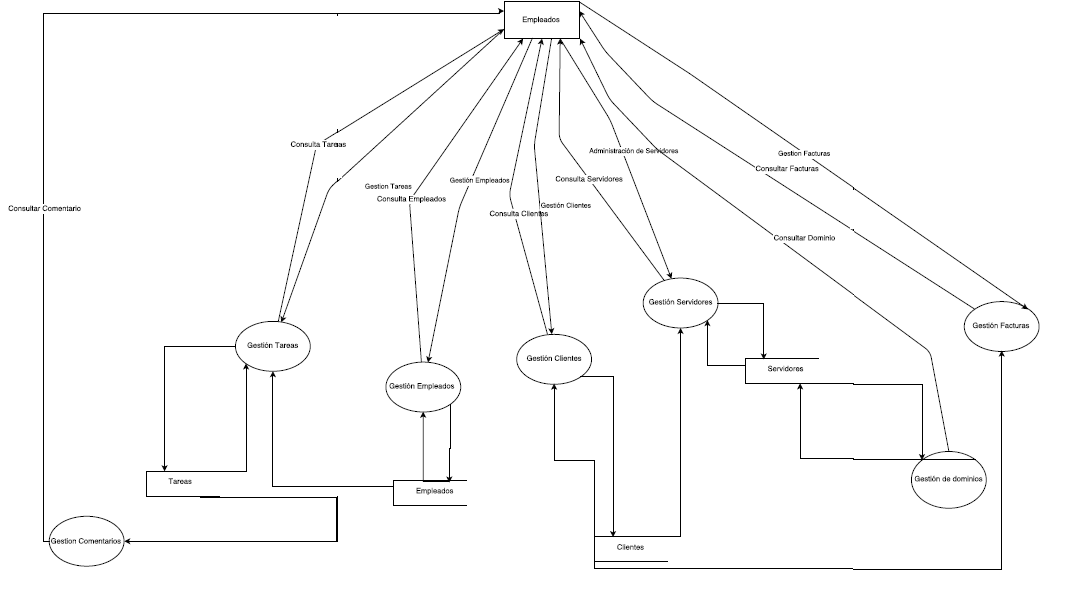
\includegraphics[width=1.25\textwidth]{SegundoRefF.png}
	\caption{}
	\label{fig:SegundoRefF}
\end{figure}

\begin{figure}
	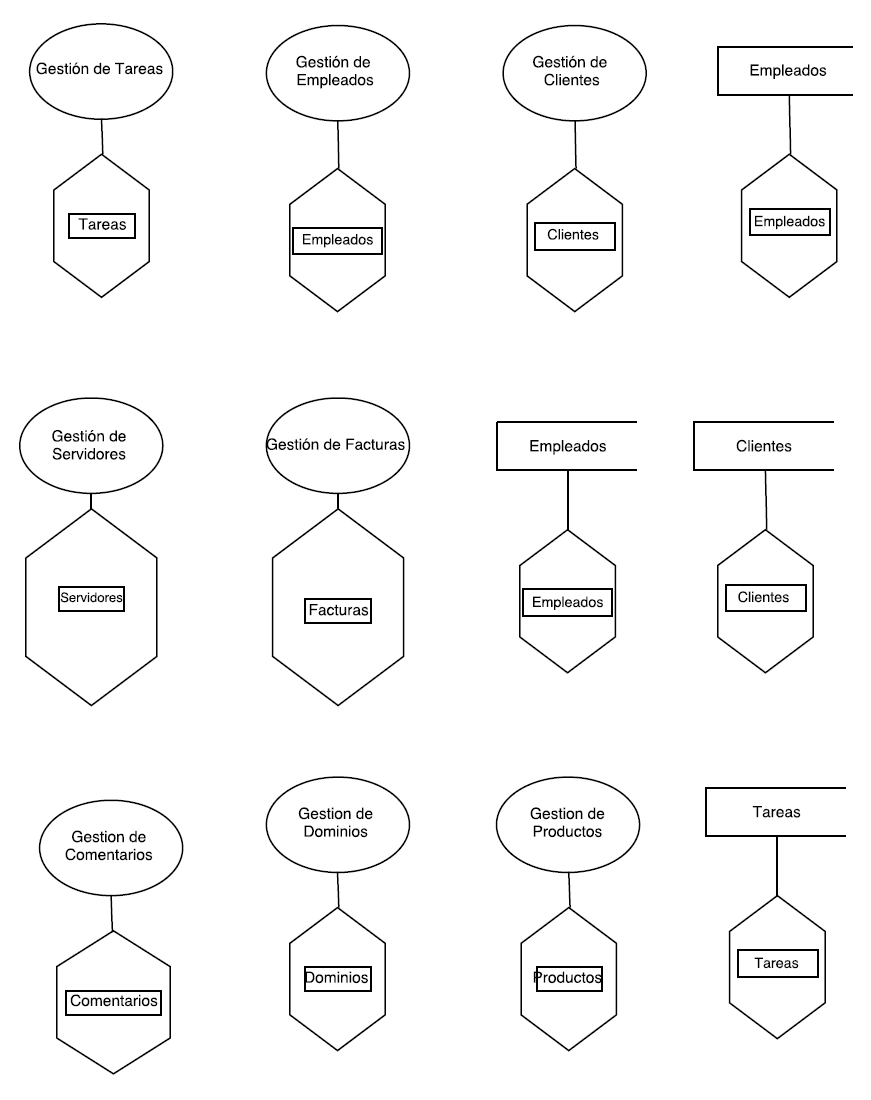
\includegraphics[width=1.20\textwidth]{EsqExtF_2.png}
	\caption{}
	\label{fig:EsqExtF_2}
\end{figure}

\begin{figure}
	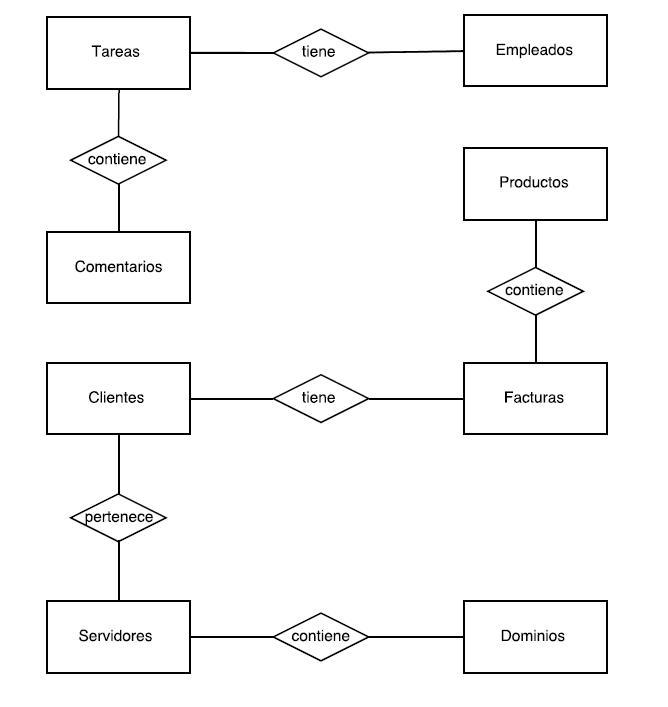
\includegraphics[width=1.20\textwidth]{SegundoRefD.png}
	\caption{}
	\label{fig:SegundoRefD}
\end{figure}

\begin{figure}
	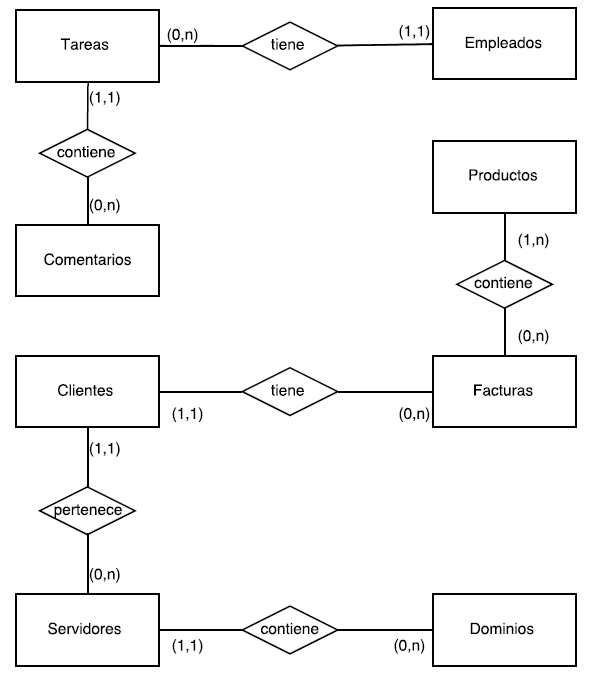
\includegraphics[width=1.20\textwidth]{PlanoFinal.png}
	\caption{}
	\label{fig:PlanoFinal}
\end{figure}


\end{document}
